%
% teil3.tex -- Beispiel-File für Teil 3
%
% (c) 2020 Prof Dr Andreas Müller, Hochschule Rapperswil
%
% !TEX root = ../../buch.tex
% !TEX encoding = UTF-8
%
\section{Luftwiderstand\label{ueberschall:section:Luftwiderstand}}
\kopfrechts{Luftwiderstand}
Der Luftwiderstand im Unterschall- und im Überschallbereich 
beruht auf unterschiedlichen physikalischen Mechanismen.
Die Luftwiderstandskraft $F_W$~\cite{StroemwiderWikiDE} eines Körpers 
berechnet sich zu
\begin{align*}
    F_W
    = c_W \, Q \, \frac{1}{2} \rho V^2,
\end{align*}
wobei $c_W$ den Luftwiderstandskoeffizienten, $Q$ die angeströmte 
Bezugsfläche und $\tfrac{1}{2}\rho V^2$ den bereits bekannten dynamischen Druck, 
präziser den Staudruck, bezeichnet.
Im Unterschall entsteht der Widerstand hauptsächlich durch die Druckverteilung 
infolge der Umströmung des Körpers. 
Im Überschall hingegen dominiert der sogenannte Wellenwiderstand, 
dessen Berechnung vergleichsweise einfach ist.
In beiden Fällen käme auch der Reibungswiderstand noch hinzu,
aber der ist hier vernachlässigbar.

Der Wellenwiderstand entsteht beim Durchbrechen 
der Schallmauer, wobei ein Teil der Bewegungsenergie 
des Körpers in die Ausbildung von sichtbaren Schockwellen übergeht,
auch bezeichnet als machsche Kegel.
An den Schattenbildern der zuvor diskutierten Projektile 
erkennt man deutlich,
wie sich Schockwellen an der Spitze und am Heck 
in kegelförmiger Strukturen ausbilden.
\begin{figure}
    \centering
    \begin{minipage}[b]{0.32\textwidth}
        \centering
        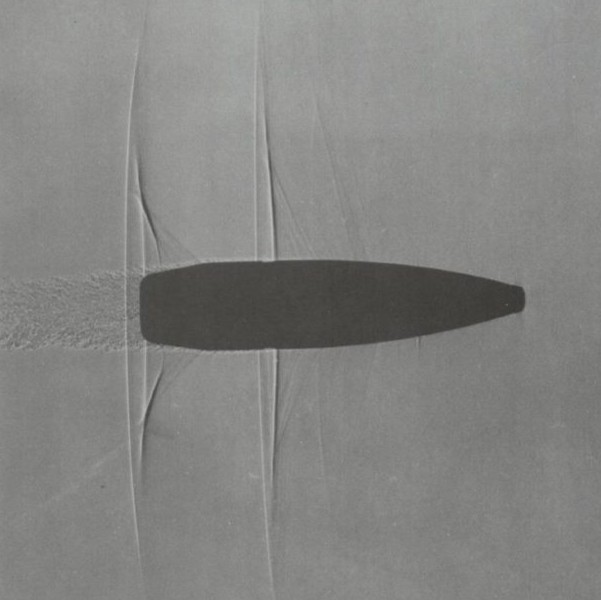
\includegraphics[width=\linewidth]{papers/ueberschall/figures/0.96_mach_projektil.jpg}
        \caption*{$0.96\,\mathrm{Mach}$}
    \end{minipage}
    \hfill
    \begin{minipage}[b]{0.32\textwidth}
        \centering
        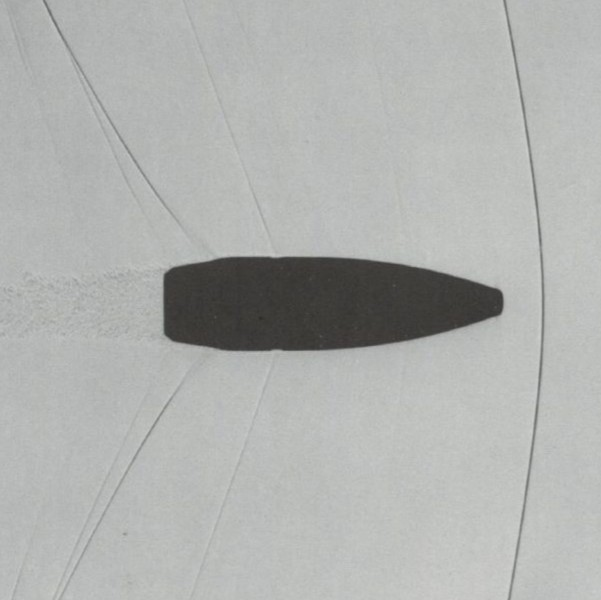
\includegraphics[width=\linewidth]{papers/ueberschall/figures/1.06_mach_projektil.jpg}
        \caption*{$1.06\,\mathrm{Mach}$}
    \end{minipage}
    \hfill
    \begin{minipage}[b]{0.32\textwidth}
        \centering
        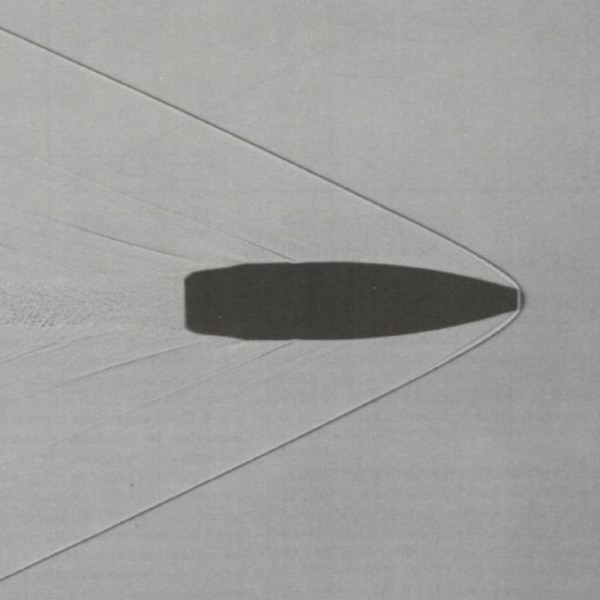
\includegraphics[width=\linewidth]{papers/ueberschall/figures/2.66_mach_projektil.jpg}
        \caption*{$2.66\,\mathrm{Mach}$}
    \end{minipage}
    \caption{Schattenbild von .50 Kaliber M33-Projektile für unterschiedliche Geschwindigkeiten~\cite{Mittelkaliber2020}.}
~\label{fig:machsche_kegel_projektil}
\end{figure}
Man erkennt bereits am ganz links dargestellten Projektil, 
das die Schallgeschwindigkeit noch nicht vollständig 
erreicht hat, die nahezu senkrechten Linien. 
Dies liegt daran, dass die umströmende Luft entlang 
des Projektils schneller ist als das Projektil selbst. 
Dadurch wird lokal die Schallgeschwindigkeit überschritten, 
was zur Ausbildung von Schockwellen führt.

Wenn wir mithilfe der Strömungsgleichungen die Druckverteilung genauer analysieren, 
lässt sich daraus auch das Verhalten des Luftwiderstands ableiten, 
wie in Abbildung~\ref{fig:luftwiderstand} qualitativ dargestellt.
\begin{figure}
    \centering
    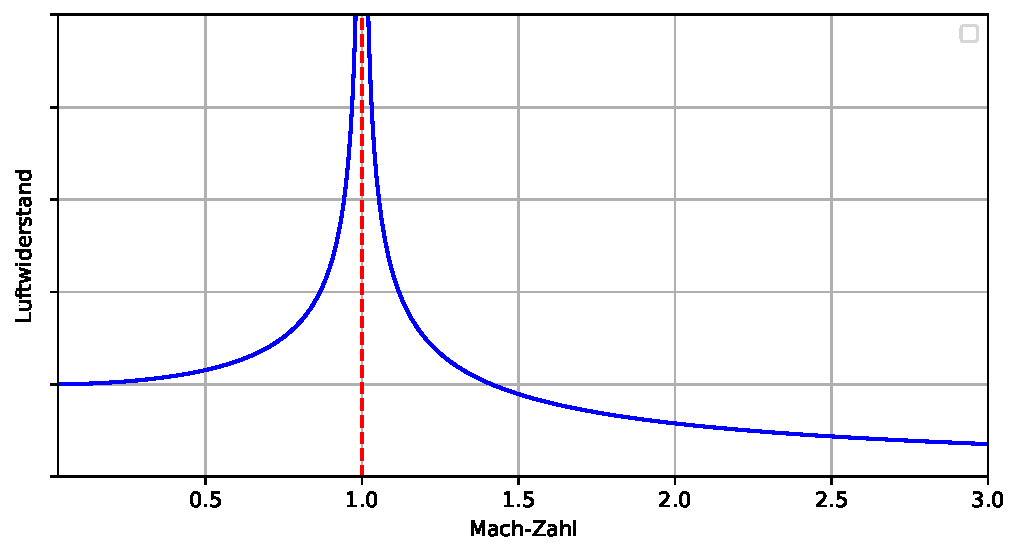
\includegraphics[width=0.8\textwidth]{papers/ueberschall/figures/Luftwiderstand_qual.pdf}
    \caption{Qualitativer Verlauf von $F_W$ und $c_W$ im Unterschall-, transsonischer und Überschallbereich.}
    \label{fig:luftwiderstand}
\end{figure}
Dabei wird schnell ersichtlich, dass diese theoretische 
Betrachtung nicht ganz der Wahrheit entspricht.
Insbesondere um den transsonischen Bereich herum, welcher rot gefärbt ist.
Gemäss den zugrunde liegenden Formeln müsste eine 
unendliche Kraft aufgebracht werden, 
um die Schallgeschwindigkeit zu erreichen — ein Widerspruch zur Tatsache, 
dass moderne Flugzeuge diese Grenze bereits überschritten haben.
Dies erklärt auch, warum in Abbildung~\ref{fig:abklingen_stromlinie} 
bei Geschwindigkeiten nahe der Schallgeschwindigkeit die Krümmung 
der Stromlinien kaum abklingt.
Es sei daher erneut betont, dass es sich bei den hier 
dargestellten Lösungen um idealisierte Näherungen handelt,
da für die exakte kompressible Strömungsgleichung bislang 
keine geschlossene Lösung bekannt ist 
(vgl. z.\,B. Gleichung~(5) aus~\cite{Ackeret1928}).
Nichtsdestotrotz beschreibt die Näherung das qualitative Verhalten korrekt:
Die Widerstandskraft $F_W$ wächst im Unterschallbereich quadratisch mit 
der Geschwindigkeit, während sie im Überschall nur noch linear zunimmt. 
Dies liegt daran, dass der Widerstandskoeffizient $c_W$ im Unterschall 
näherungsweise konstant bleibt, im Überschall 
jedoch mit $1/M$ abnimmt.

Zur Veranschaulichung dieses Effekts wird nun ein reales Beispiel 
mit empirisch ermittelten Daten herangezogen:
Ein Projektil des Typs $.50\,\text{BMG}$ M33.
Abbildung~\ref{fig:luftwiderstand_50-M33}(b) zeigt den Verlauf
des Luftwiderstands über der Mach-Zahl.
Dabei ist deutlich zu erkennen, dass der Luftwiderstand 
im Übergang von Unterschall zu Überschall 
deutlich ansteigt und nach dem Überschreiten der 
Schallgeschwindigkeit bei etwa $1.2\,\text{Mach}$ 
wieder abnimmt.
Die Vorgänge im transsonischen Bereich sind bis heute 
nicht vollständig geklärt.
\begin{figure}
    \centering
    \begin{minipage}[t]{0.4\textwidth}
        \centering
        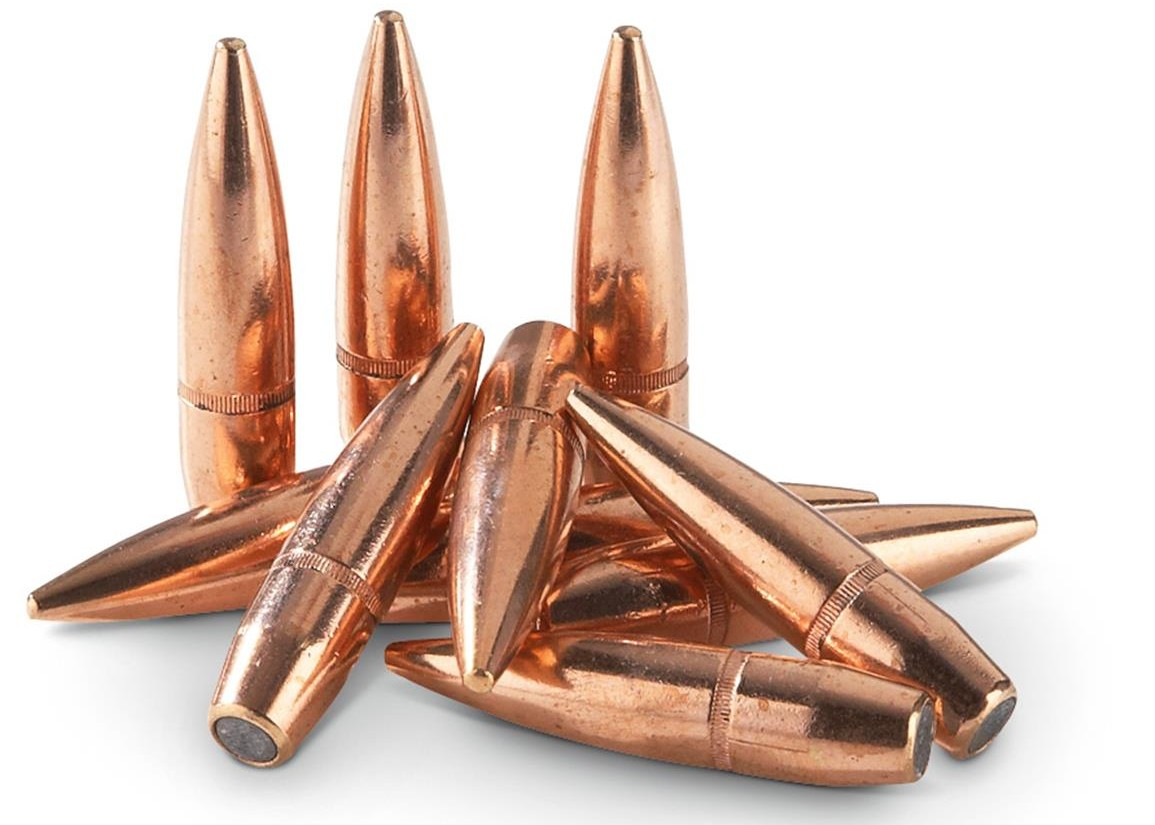
\includegraphics[width=\linewidth]{papers/ueberschall/figures/50-cal_projectile.jpg}
        \caption*{(a) $.50\,\text{BMG}$ M33-Projektil~\cite{ArmoryFarm50BMG}.}
    \end{minipage}
    \hfill
    \begin{minipage}[t]{0.55\textwidth}
        \centering
        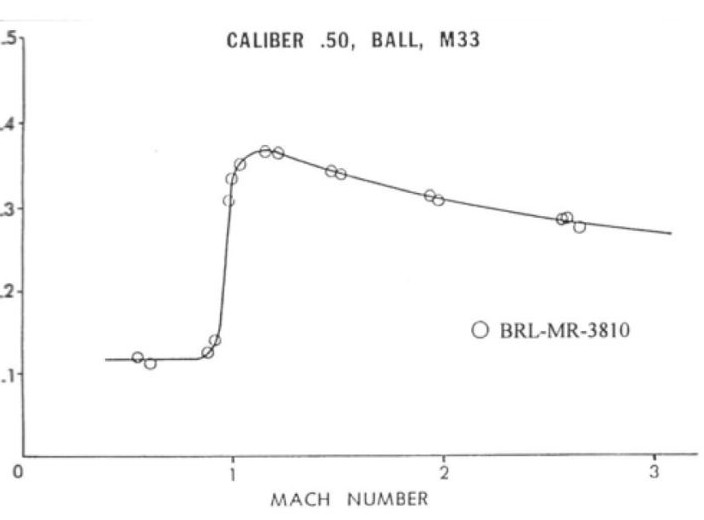
\includegraphics[width=\linewidth]{papers/ueberschall/figures/50-M33 Geschoss.jpg}
        \caption*{(b) Luftwiderstandskoeffizient $c_W$ als Funktion der Machzahl~\cite{Mittelkaliber2020}.}
    \end{minipage}
    \caption{Projektil und Luftwiderstandskurve.}
    ~\label{fig:luftwiderstand_50-M33}
\end{figure}

\subsection{Sears-Haack-Körper}
Die Minimierung des Luftwiderstands im Überschallbereich 
gestaltet sich deutlich einfacher als im Unterschall. 
Einen Körper zu finden, der sowohl im Unterschall-, 
transsonischen als auch im Überschallbereich optimal ist, 
erweist sich aufgrund der unterschiedlichen 
Strömungsmechaniken als kaum möglich.
Daher beschränken wir uns im Folgenden auf den einfachsten Fall.
Der Sears-Haack-Körper, illustriert in Abbildung~\ref{fig:sears_haack}(a), 
besitzt den theoretisch geringsten Wellenwiderstand. 
Im Bereich von etwa $1.5$ bis $3\,\mathrm{Mach}$ 
stellt er die strömungsgünstigste Form dar. 
Wolfgang Haack bestimmte diese Form mithilfe eines 
Variationsprinzips und legte die ausführliche Herleitung 
in~\cite{Haack1941} vor.
\begin{figure}
    \centering
    \begin{minipage}[t]{0.48\textwidth}
       \centering
        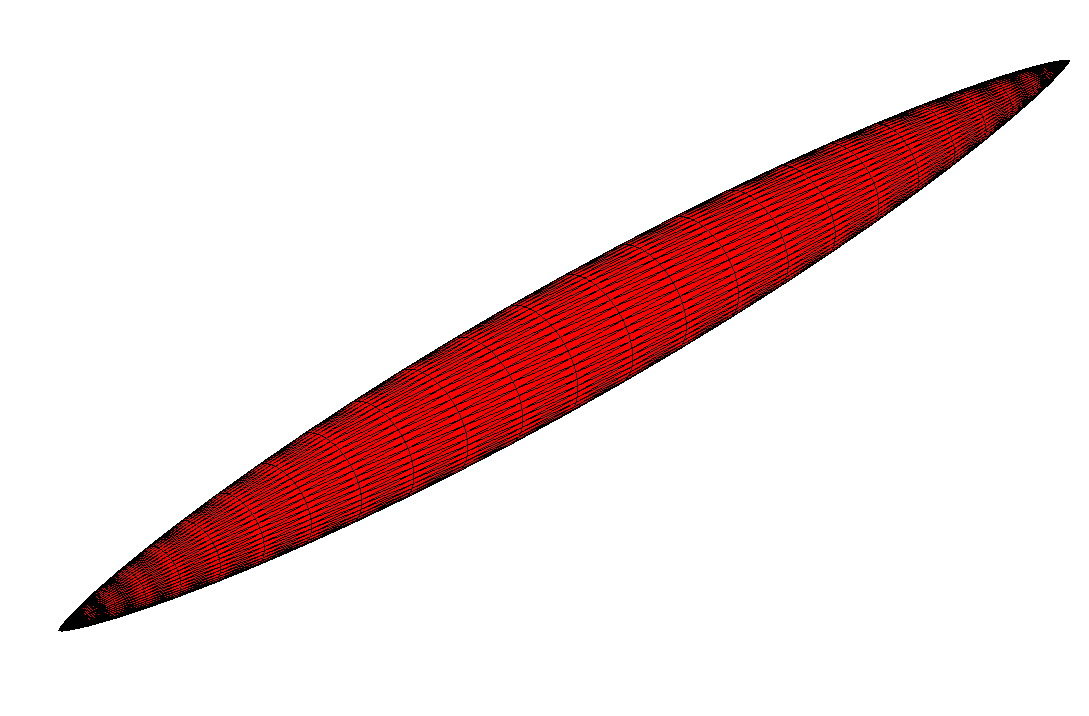
\includegraphics[height=4.5cm]{papers/ueberschall/figures/Sears-Haack.png}
        \caption*{(a) Sears-Haack-Körper~\cite{SearsHaackWikipedia}}
    \end{minipage}
    \hfill
    \begin{minipage}[t]{0.48\textwidth}
        \centering
        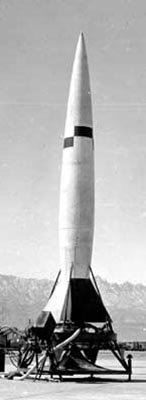
\includegraphics[height=6cm]{papers/ueberschall/figures/hermes-a3a.jpg}
        \caption*{(b) Hermes A-3A~\cite{WeebauHermesA3A}}
    \end{minipage}
    \caption{Körper mit minimalem Luftwiderstand und die Anwendung in der Luftfahrt.}
    ~\label{fig:sears_haack}
\end{figure}
Haacks ursprüngliches Ziel war die Optimierung von Scharfschützengewehren. 
Praktische Gründe führten jedoch dazu, dass diese 
Form nicht verwendet wurde. 
Stattdessen erfolgte die Optimierung der Projektile 
durch einen Heckkonus, wie in Abbildung~\ref{fig:luftwiderstand_50-M33}(a) ersichtlich.
Nichtsdestotrotz hat der Sears-Haack-Körper aufgrund 
seiner strömungsoptimierten Form eine große Bedeutung 
für die Gestaltung von Flugkörpern und Raketen
im Überschallbereich erlangt.
Ein gutes Beispiel dafür ist die Hermes A-3A, siehe Abbildung~\ref{fig:sears_haack}(b).